% !TEX encoding = UTF-8
% !TEX TS-program = pdflatex
% !TEX root = ../Tesi.tex
% !TEX spellcheck = it-IT

\clearpage

\section{Attore gestore della squadra}
%
% Figura: casi d'uso dell'attore gestore della squadra
%
\begin{figure}[h]
	\centering
	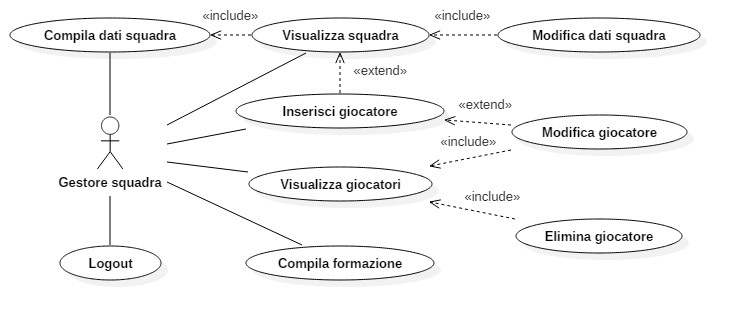
\includegraphics[width=0.8\textwidth]
	{immagini/uc-gestore-squadra}
	
	\caption{Casi d'uso dell'attore gestore della squadra}
\end{figure}


%
% Caso d'uso: Logout
%
\subsection{Caso d'uso: Logout}

\subsubsection*{Descrizione}
Questa funzionalità permette al gestore della squadra di uscire dalla sua pagina e di iniziare a navigare come utente pubblico.
Il pulsante di Logout è presente in ogni pagina dell'applicazione web, in alto a destra.

\subsubsection*{Attori coinvolti}
Gestore della squadra, partecipazione attiva dell'attore verso il caso d'uso medesimo.

\subsubsection*{Pre-condizioni}
È richiesto l'accesso al sistema tramite la funzionalità di login.

\subsubsection*{Post-condizioni}
Termina la sessione di accesso al sistema in qualità di gestore della squadra.

\subsubsection*{Flusso principale}

\begin{enumerate}
	
	\item
	Il gestore della squadra seleziona nella pagina in cui si trova il pulsante di Logout;
	
	\item
	Il sistema scollega l'amministratore dalle pagine a lui riservate;
	
	\item
	Il sistema redireziona il gestore della squadra nella schermata di login e da quel momento può navigare come utente pubblico.
	
\end{enumerate}

\subsubsection*{Flussi alternativi}
Nel caso di operazione non riuscita si notifica all'amministratore il tipo di errore che si è verificato.

\subsection*{Diagramma delle attività}
Il diagramma delle attività per il caso d'uso ``Logout'' è illustrato nella figura \vref{ad-logout}.

%
% Caso d'uso: Inserisci giocatore
%
\subsection{Caso d'uso: Inserisci giocatore}
\label{uc-inserisci-giocatore}

\subsubsection*{Descrizione}
Questa funzionalità permette al gestore squadra di inserire nella rosa della propria squadra un nuovo giocatore.

\subsubsection*{Attori coinvolti}
Gestore squadra, partecipazione attiva dell'attore verso il caso d'uso medesimo.
Il gestore squadra interagisce direttamente con il sistema compilando i campi richiesti.

\subsubsection*{Pre-condizioni}
È richiesto l'accesso al sistema come gestore squadra, tramite la funzionalità di login, in quanto solo lui può inserire un nuovo giocatore nella sua squadra. Il gestore squadra può inserire al massimo 36 giocatori.

\subsubsection*{Post-condizioni}
Viene aggiornato lo stato sul database con l'inserimento di un nuovo giocatore.

\subsubsection*{Flusso principale}

\begin{enumerate}
	
	\item
	Il gestore squadra seleziona la voce ``Nuovo Giocatore'' nella propria home page oppure seleziona la voce ``Inserisci Nuovo Giocatore'' nella pagina di visualizzazione della squadra oppure seleziona la voce ``Inserisci Nuovo Giocatore'' nella pagina di visualizzazione dei giocatori;
	
	\item
	Il gestore squadra inserisce per il giocatore i seguenti dati: nome, cognome, data di nascita, nazionalità, numero di maglia, ruolo, foto e descrizione;
	
	\item
	Il gestore squadra invia la richiesta di creazione del nuovo giocatore al sistema;
	
	\item
	Il sistema controlla che il gestore della squadra abbia inserito correttamente tutti i dati. Se i dati sono corretti il sistema crea un nuovo giocatore;
	
	\item
	Il sistema visualizza i dati del giocatore appena inserito dando la possibilità al gestore della squadra di modificarli;
	
\end{enumerate}

\subsubsection*{Flussi alternativi}
Nel caso di operazione non riuscita, si notifica al gestore della squadra il tipo di errore che si è verificato.


%
% Caso d'uso: Elimina giocatore
%
\subsection{Caso d'uso: Elimina giocatore}

\subsubsection*{Descrizione}
Questa funzionalità permette al gestore della squadra di eliminare un giocatore dalla rosa della squadra che gestisce.

\subsubsection*{Attori coinvolti}
Gestore squadra, partecipazione attiva dell'attore verso il caso d'uso medesimo.
Il gestore squadra interagisce direttamente con il sistema eliminando il giocatore selezionato.

\subsubsection*{Pre-condizioni}
È richiesto l'accesso al sistema come gestore squadra, tramite la funzionalità di login, in quanto solo lui ha il privilegio di poter eliminare i propri giocatori.

\subsubsection*{Post-condizioni}
Viene aggiornato lo stato sul database con l'eliminazione del giocatore selezionato.

\subsubsection*{Flusso principale}

\begin{enumerate}
	
	\item
	Il gestore della squadra seleziona la voce ``Elimina'', per il giocatore che desidera eliminare, nella lista dei giocatori;
	
	\item
	Il sistema chiede la conferma di esecuzione dell'operazione;
	
	\item
	Se il gestore della squadra conferma l'operazione il giocatore viene eliminato altrimenti l'operazione viene annullata.
	
\end{enumerate}

\subsubsection*{Flussi alternativi}
Nel caso di operazione non riuscita, si notifica al gestore della squadra il tipo di errore che si è verificato.

\subsubsection*{Punti di inclusione}
Si può accedere a questo caso d'uso quando si effettua la visualizzazione di tutti i giocatori, vedi caso d'uso \vref{uc-visualizza-giocatori}.


%
% Caso d'uso: Visualizza giocatori
%
\subsection{Caso d'uso: Visualizza giocatori}
\label{uc-visualizza-giocatori}

\subsubsection*{Descrizione}
Questa funzionalità permette di visualizzare la lista di tutti gli i giocatori creati da un gestore di una squadra.

\subsubsection*{Attori coinvolti}
Gestore squadra, partecipazione attiva dell'attore verso il caso d'uso medesimo.

\subsubsection*{Pre-condizioni}
È richiesto l'accesso al sistema come gestore squadra, tramite la funzionalità di login.

\subsubsection*{Post-condizioni}
Nessuna post-condizione in quanto la visualizzazione dei giocatori non contribuisce a cambiare lo stato del sistema.

\subsubsection*{Flusso principale}

\begin{enumerate}
	
	\item
	Il gestore della squadra seleziona la voce ``Giocatori'' nella pagina in cui si trova;
	
	\item
	Il sistema visualizza tutti i giocatori in ordine alfabetico mostrandone: foto, nome, cognome, numero maglia e ruolo. Il sistema, inoltre, visualizza per ogni utente un pulsante per eliminare l'utente e il pulsante per modificare l'utente.
	
\end{enumerate}

\subsubsection*{Flussi alternativi}
Nel caso di operazione non riuscita, si notifica al gestore della squadra il tipo di errore che si è verificato.


%
% Caso d'uso: Visualizza squadra
%
\subsection{Caso d'uso: Visualizza squadra}
\label{uc-visualizza-squadra}

\subsubsection*{Descrizione}
Questa funzionalità permette al gestore della squadre di visualizzare la propria squadra.

\subsubsection*{Attori coinvolti}
Gestore squadra, partecipazione attiva dell'attore verso il caso d'uso medesimo.

\subsubsection*{Pre-condizioni}
È richiesto l'accesso al sistema come gestore squadra, tramite la funzionalità di login.

\subsubsection*{Post-condizioni}
Nessuna post-condizione in quanto la visualizzazione della squadra non contribuisce a cambiare lo stato del sistema.

\subsubsection*{Flusso principale}

\begin{enumerate}
	
	\item
	Il gestore della squadra seleziona la voce ``Visualizza Squadra'' nella sua home page oppure seleziona nella pagina in cui si trova la voce ``Squadra'';
	
	\item
	Il sistema visualizza i dati della squadra mostrandone: nome, logo, immagine della squadra, sede, descrizione, nome dello sponsor e logo dello sponsor.
	
\end{enumerate}

\subsubsection*{Flussi alternativi}
Nel caso il gestore della squadra non abbia compilato i dati della squadra si attiva il caso d'uso Compila squadra, vedi caso d'uso \vref{uc-compila-squadra}.

Nel caso di operazione non riuscita, si notifica al gestore della squadra il tipo di errore che si è verificato.


%
% Caso d'uso: Modifica squadra
%
\subsection{Caso d'uso: Modifica squadra}
\label{uc-modifica-squadra}

\subsubsection*{Descrizione}
Questa funzionalità permette al gestore squadra di modificare i dati della propria squadra.

\subsubsection*{Attori coinvolti}
Gestore squadra, partecipazione attiva dell'attore verso il caso d'uso medesimo.
Il gestore squadra interagisce direttamente con il sistema compilando i campi richiesti.

\subsubsection*{Pre-condizioni}
È richiesto l'accesso al sistema come gestore squadra, tramite la funzionalità di login, in quanto solo lui può modificare i dati della sua squadra.

\subsubsection*{Post-condizioni}
Viene aggiornato lo stato sul database con l'aggiornamento dei dati di una squadra.

\subsubsection*{Flusso principale}

\begin{enumerate}
	
	\item
	Il gestore della squadra seleziona la voce ``Modifica'' nella pagina di visualizzazione della squadra oppure seleziona la voce ``Inserisci Nuovo Giocatore'' nella pagina di visualizzazione dei giocatori;
	
	\item
	Il gestore della squadra inserisce per la squadra i seguenti dati: nome, sede, foto della squadra, logo della squadra, nome dello sponsor, immagine dello sponsor e descrizione della squadra;
	
	\item
	Il gestore della squadra seleziona la voce ``Conferma Modifiche'';
	
	\item
	Il sistema controlla che il gestore della squadra abbia inserito correttamente tutti i dati. Se i dati sono corretti il sistema invia una richiesta di conferma dei dati inseriti al gestore della squadra;
	
	\item
	Se il gestore della squadra conferma la modifica allora il sistema visualizza la pagina della squadra con i dati aggiornati;
	
\end{enumerate}

\subsubsection*{Flussi alternativi}
Nel caso di operazione non riuscita, si notifica al gestore della squadra il tipo di errore che si è verificato.

\subsection*{Diagramma delle attività}
Il diagramma delle attività per il caso d'uso ``Modifica squadra'' è illustrato nella figura \vref{ad-modifica-squadra}.


%
% Figura: diagramma delle attività relativo alla creazione del torneo all'italiana
%
\begin{figure}[h]
	\centering
	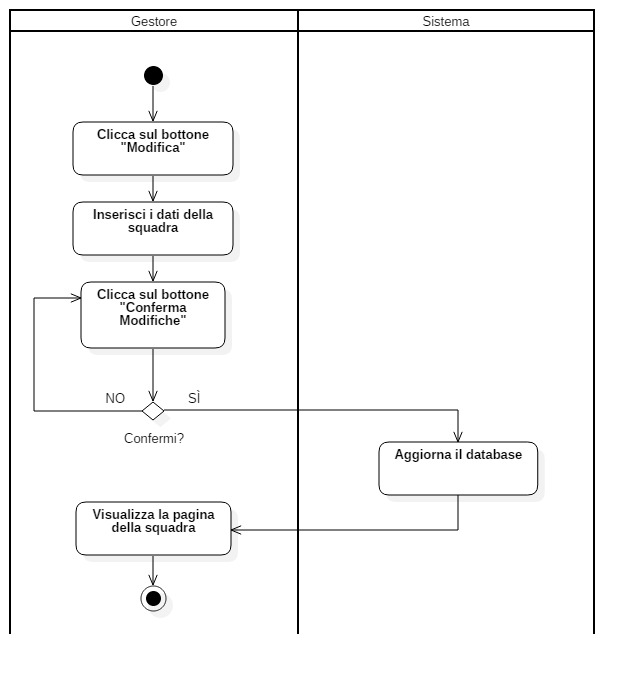
\includegraphics[width=0.8\textwidth]
	{immagini/ad-modifica-squadra}
	
	\caption{Diagramma delle attività di modifica della squadra}
	\label{ad-modifica-squadra}
\end{figure}


%
% Caso d'uso: Compila formazione
%
\subsection{Caso d'uso: Compila formazione}

\subsubsection*{Descrizione}
Questa funzionalità permette al gestore squadra di scegliere i giocatori che faranno parte ad una formazione in una determinata partita.

\subsubsection*{Attori coinvolti}
Gestore squadra, partecipazione attiva dell'attore verso il caso d'uso medesimo.

Il gestore squadra interagisce direttamente con il sistema scegliendo 11 giocatori titolari e 7 riserve.

\subsubsection*{Pre-condizioni}
È richiesto l'accesso al sistema come gestore squadra, tramite la funzionalità di login, in quanto solo lui può compilare la formazione per una partita.

\subsubsection*{Post-condizioni}
Viene aggiornato lo stato sul database con l'inserimento della formazione scelta dal gestore della squadra.

\subsubsection*{Flusso principale}

\begin{enumerate}
	
	\item
	Il gestore della squadra seleziona la voce ``Nuova Formazione'' nella propria home page oppure seleziona la voce ``Formazioni'' nella pagina di visualizzazione dei giocatori;
	
	\item
	Il sistema visualizza la lista di tutte le partite a cui il gestore deve fornire la formazione dove per ogni partita vengono visualizzate le seguenti informazioni: id del referto, nome del torneo, le due squadre sfidanti e la data della partita. Il sistema, inoltre, visualizza per ogni partita un pulsante per compilare la formazione della squadra per la partita corrispondente;
	
	\item
	Il gestore della squadra seleziona una partita;
	
	\item
	Il sistema visualizza la lista di tutti i giocatori che fanno parte della squadra con a lato la possibilità di scegliere se far giocare un giocatore come titolare o come riserva;
	
	\item
	Il gestore della squadra sceglie 11 giocatori titolari e 7 giocatori riserve;
	
	\item
	Il gestore seleziona la voce ``Conferma Formazione'';
	
	\item
	Il sistema controlla che il gestore della squadra abbia selezionato correttamente i giocatori. Se i giocatori sono stati selezionati correttamente il sistema invia una richiesta di conferma della formazione inserita al gestore della squadra altrimenti invia una notifica dell'errore commesso al gestore della squadra;
	
	\item
	Se il gestore della squadra conferma la formazione allora il sistema aggiorna il database inserendo la formazione appena compilata e visualizza la lista di tutte le partite rimanenti a cui il gestore deve fornire la formazione;
	
\end{enumerate}

\subsubsection*{Flussi alternativi}
Nel caso di operazione non riuscita, si notifica al gestore della squadra il tipo di errore che si è verificato.